\documentclass[11pt]{article}
\usepackage[utf8]{inputenc}
\usepackage[T1]{fontenc}
\usepackage{amsmath}
\usepackage{amssymb}
\usepackage{multicol}
\usepackage{geometry}
\usepackage{tikz}
\usepackage{enumitem}
\usepackage{xcolor}
\usepackage{titlesec}
\usepackage{pgfplots}
\pgfplotsset{compat=1.18}

% Configurações de layout
\geometry{a4paper, left=1cm, right=1cm, top=0.5cm, bottom=1.2cm}
\setlength{\columnseprule}{0.4pt}

% Cores para títulos
\titleformat{\section}{\normalfont\Large\bfseries\color{blue}}{\thesection}{1em}{}
\titleformat{\subsection}{\normalfont\large\bfseries\color{red}}{\thesubsection}{1em}{}

% Comandos personalizados
\newcommand{\respostaNum}[1]{\textcolor{blue}{\boxed{#1}}}   % para números
\newcommand{\respostaTxt}[1]{\textcolor{blue}{#1}}           % para textos
\newcommand{\resolucao}{\textbf{\textcolor{blue}{Resolução:}}}
\newcommand{\atencao}{\textbf{\textcolor{red}{Atenção!}}}

\title{\textcolor{green}{Gabarito Comentado: Introdução à Estatística}}
\author{Professor: Jefferson}
\date{}

\begin{document}

\maketitle
\vspace{-1cm}

\begin{multicols}{2}

\section*{Instruções}
\textbf{Verifique suas respostas e estude as resoluções comentadas.}

\section*{Gabarito - Exercícios Básicos}

\begin{enumerate}[leftmargin=*]

\item \textbf{Classifique as variáveis:}

\begin{enumerate}[label=\alph*)]
\item Número de irmãos

\resolucao Quantitativa discreta (valores inteiros: 0, 1, 2, \ldots)

\respostaTxt{Quantitativa Discreta}

\item Cor dos olhos

\resolucao Qualitativa nominal (sem ordem: azul, castanho, verde, \ldots)

\respostaTxt{Qualitativa Nominal}

\item Temperatura corporal

\resolucao Quantitativa contínua (pode assumir valores decimais: 36,5°C, 37,2°C)

\respostaTxt{Quantitativa Contínua}

\item Nível de satisfação (bom, regular, ruim)

\resolucao Qualitativa ordinal (possui ordem natural entre as categorias)

\respostaTxt{Qualitativa Ordinal}

\item Salário mensal

\resolucao Quantitativa contínua (pode assumir qualquer valor real positivo)

\respostaTxt{Quantitativa Contínua}

\item Marca de celular

\resolucao Qualitativa nominal (sem ordem: Samsung, Apple, Motorola, \ldots)

\respostaTxt{Qualitativa Nominal}
\end{enumerate}

\item \textbf{Dados as idades: 18, 20, 22, 18, 25, 20, 18, 22}

\begin{enumerate}[label=\alph*)]
\item Construa a tabela de frequência

\resolucao Ordenando os dados: 18, 18, 18, 20, 20, 22, 22, 25

\[
\begin{array}{|c|c|c|c|}
\hline
\textbf{Idade} & \textbf{Contagem} & \boldsymbol{f_i} & \boldsymbol{fr_i} \\
\hline
18 & III & 3 & 3/8 = 0,375 \\
20 & II & 2 & 2/8 = 0,250 \\
22 & II & 2 & 2/8 = 0,250 \\
25 & I & 1 & 1/8 = 0,125 \\
\hline
\text{Total} & & 8 & 1,000 \\
\hline
\end{array}
\]

\respostaTxt{Tabela construída acima}

\item Calcule frequência relativa

\resolucao
\[
fr_{18} = \frac{3}{8} = \respostaNum{0,375}, \quad
fr_{20} = \frac{2}{8} = \respostaNum{0,250}, \quad
\]
\[ fr_{22} = \frac{2}{8} = \respostaNum{0,250}, \quad
fr_{25} = \frac{1}{8} = \respostaNum{0,125}
\]

\item Qual a moda?

\resolucao O valor que mais aparece é 18 (3 ocorrências)

\respostaTxt{Mo = 18 anos}
\end{enumerate}

\item \textbf{As notas de 10 alunos foram: 5, 6, 7, 8, 5, 6, 9, 7, 6, 8}

\begin{enumerate}[label=\alph*)]
\item Calcule a média

\resolucao
\[
    \bar{x} = \frac{5 + 6 + 7 + 8 + 5 + 6 + 9 + 7 + 6 + 8}{10} \]
\[= \frac{67}{10} = \respostaNum{6,7}
\]

\item Encontre a mediana

\resolucao Ordenando os dados: 5, 5, 6, 6, 6, 7, 7, 8, 8, 9
\[
Md = \frac{6 + 7}{2} = \frac{13}{2} = \respostaNum{6,5}
\]

\item Determine a moda

\resolucao O valor que mais aparece é 6 (três ocorrências)

\respostaTxt{Mo = 6}
\end{enumerate}

\item \textbf{Complete a tabela:}

\begin{center}
\begin{tabular}{|c|c|c|c|}
\hline
\textbf{Notas} & \textbf{$f_i$} & \textbf{$fr_i$} & \textbf{\%} \\
\hline
0-2 & 3 & 0,10 & 10\% \\
2-4 & 5 & 0,166... & 16,67\% \\
4-6 & 8 & 0,266... & 26,67\% \\
6-8 & 10 & 0,333... & 33,33\% \\
8-10 & 4 & 0,133... & 13,33\% \\
\hline
Total & 30 & 1,00 & 100\% \\
\hline
\end{tabular}
\end{center}

\resolucao
\[
fr_i = \frac{f_i}{30}, \quad \% = fr_i \times 100\%
\]
\respostaTxt{Tabela completa acima}

\item \textbf{Problemas contextualizados:}

\begin{enumerate}[label=\alph*)]
\item Em uma pesquisa com 50 pessoas sobre time de futebol: 32 torcem para o time A, 12 para o time B e 6 para o time C. Construa o gráfico de setores.

\resolucao Cálculo dos ângulos:
\[
 \text{Time A: } 32 \times \frac{360°}{50} = 230,4° \quad \] 
\[\text{Time B: } 12 \times \frac{360°}{50} = 86,4° \quad \]
\[\text{Time C: } 6 \times \frac{360°}{50} = 43,2°
\]
\respostaTxt{Gráfico com setores de 230,4° (64\%), 86,4° (24\%) e 43,2° (12\%)}

\item As temperaturas máximas de uma semana foram: 28°, 30°, 29°, 31°, 32°, 30°, 29°C. Calcule a temperatura média.

\resolucao
\[
\bar{x} = \frac{28 + 30 + 29 + 31 + 32 + 30 + 29}{7} \]
\[= \frac{209}{7} \approx \respostaNum{29,86°C}
\]
\end{enumerate}

\item \textbf{Analise o histograma:}

\begin{center}
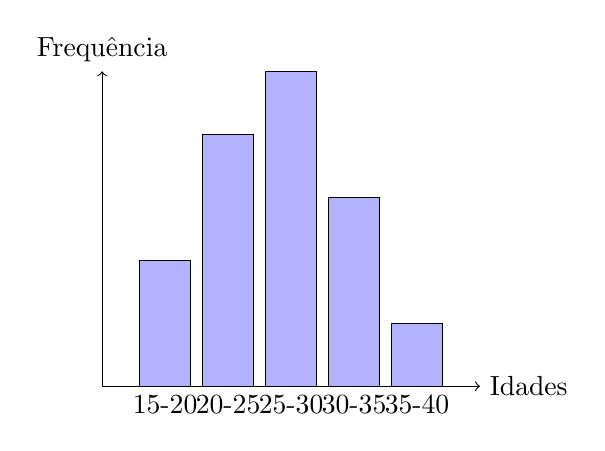
\begin{tikzpicture}[scale=0.8]
\draw[->] (0,0) -- (6,0) node[right] {Idades};
\draw[->] (0,0) -- (0,5) node[above] {Frequência};
\foreach \x/\y in {1/2, 2/4, 3/5, 4/3, 5/1}
  \draw[fill=blue!30] (\x-0.4,0) rectangle (\x+0.4,\y);
\node at (1,0) [below] {15-20};
\node at (2,0) [below] {20-25};
\node at (3,0) [below] {25-30};
\node at (4,0) [below] {30-35};
\node at (5,0) [below] {35-40};
\end{tikzpicture}
\end{center}

\begin{enumerate}[label=\alph*)]
\item Qual faixa etária tem maior frequência?

\resolucao A barra mais alta corresponde à faixa 25-30 anos (frequência 5)

\respostaTxt{25-30 anos}

\item Quantas pessoas têm entre 25 e 30 anos?

\resolucao Pelo histograma, a frequência da faixa 25-30 é 5

\respostaTxt{5 pessoas}

\item Qual o total de pessoas pesquisadas?

\resolucao Somando todas as frequências: 2 + 4 + 5 + 3 + 1 = 15

\respostaTxt{15 pessoas}
\end{enumerate}

\item \textbf{Dados agrupados:}

\begin{center}
\begin{tabular}{|c|c|}
\hline
\textbf{Salário (R\$)} & \textbf{Nº funcionários} \\
\hline
1000-1500 & 8 \\
1500-2000 & 12 \\
2000-2500 & 15 \\
2500-3000 & 10 \\
3000-3500 & 5 \\
\hline
\end{tabular}
\end{center}

\begin{enumerate}[label=\alph*)]
\item Calcule o ponto médio de cada classe

\resolucao
\[x_1 = \frac{1000+1500}{2} = \respostaNum{1250}, \quad \]
\[x_2 = \frac{1500+2000}{2} = \respostaNum{1750}, \quad \]
\[x_3 = \frac{2000+2500}{2} = \respostaNum{2250}\]
\[x_4 = \frac{2500+3000}{2} = \respostaNum{2750}, \quad \]
\[x_5 = \frac{3000+3500}{2} = \respostaNum{3250} \]

\item Calcule a média aproximada

\resolucao
\[
\bar{x} = \frac{1250 \cdot 8 + 1750 \cdot 12 + 2250 \cdot 15 + 2750 \cdot 10 + 3250 \cdot 5}{8+12+15+10+5}
\]
\[
    \bar{x} = \frac{10000 + 21000 + 33750 + 27500 + 16250}{50} \]
\[ = \frac{108500}{50} = \respostaNum{R\$ 2170,00}\]

\item Em qual classe está a mediana?

\resolucao Total = 50, mediana está na posição 25,5. Acumulando:
Classe 1: 8, Classe 2: 20, Classe 3: 35 (atinge 35, ultrapassando 25,5)

\respostaTxt{Classe 2000-2500}
\end{enumerate}

\item \textbf{Escolha o gráfico adequado:}

\begin{enumerate}[label=\alph*)]
\item Distribuição de idade em uma população

\resolucao Dados contínuos agrupados em classes $\rightarrow$ melhor é \respostaTxt{Histograma}

\item Preferência por marcas de refrigerante

\resolucao Dados qualitativos nominais $\rightarrow$ melhor é \respostaTxt{Gráfico de barras ou pizza}

\item Evolução das vendas ao longo do ano

\resolucao Dados temporais $\rightarrow$ melhor é \respostaTxt{Gráfico de linhas}

\item Composição do orçamento familiar

\resolucao Partes de um todo $\rightarrow$ melhor é \respostaTxt{Gráfico de setores (pizza)}
\end{enumerate}

\item \textbf{Pesquisa sobre meio de transporte:}

\begin{center}
\begin{tabular}{|l|c|}
\hline
\textbf{Transporte} & \textbf{Frequência} \\
\hline
Ônibus & 25 \\
Carro & 15 \\
Metrô & 20 \\
Bicicleta & 8 \\
A pé & 12 \\
\hline
Total & 80 \\
\hline
\end{tabular}
\end{center}

\begin{enumerate}[label=\alph*)]
\item Calcule as frequências relativas

\resolucao
\[
fr_{\text{Ônibus}} = \frac{25}{80} = \respostaNum{0,3125}, \quad
fr_{\text{Carro}} = \frac{15}{80} = \respostaNum{0,1875}, \quad
fr_{\text{Metrô}} = \frac{20}{80} = \respostaNum{0,25}
\]
\[
fr_{\text{Bicicleta}} = \frac{8}{80} = \respostaNum{0,10}, \quad
fr_{\text{A pé}} = \frac{12}{80} = \respostaNum{0,15}
\]

\item Construa o gráfico de barras

\resolucao Gráfico com eixo x com os transportes, eixo y com as frequências (0 a 25)

\respostaTxt{Gráfico de barras com barras nas alturas: Ônibus=25, Carro=15, Metrô=20, Bicicleta=8, A pé=12}

\item Qual a porcentagem que usa carro?

\resolucao
\[
\% = \frac{15}{80} \times 100\% = 18,75\%
\]
\respostaNum{18,75\%}
\end{enumerate}

\item \textbf{Para cada situação, indique se é população ou amostra:}

\begin{enumerate}[label=\alph*)]
\item Todos os alunos da escola

\respostaTxt{População (censo)}

\item 50 clientes sorteados de um supermercado

\respostaTxt{Amostra}

\item Todas as casas do bairro

\respostaTxt{População}

\item 1000 eleitores pesquisados

\respostaTxt{Amostra}
\end{enumerate}
\end{enumerate}

\section*{Gabarito - Exercícios Avançados}

\begin{enumerate}[leftmargin=*, start=11]

\item \textbf{Duas turmas têm as seguintes médias:}
\begin{itemize}
\item Turma A: $\bar{x} = 7,2$ com 30 alunos
\item Turma B: $\bar{x} = 6,8$ com 25 alunos
\end{itemize}
Qual a média geral das duas turmas juntas?

\resolucao
\[
\bar{x}_{\text{geral}} = \frac{30 \cdot 7,2 + 25 \cdot 6,8}{30 + 25} = \frac{216 + 170}{55} = \frac{386}{55} \approx \respostaNum{7,02}
\]

\item \textbf{Construa a ogiva para os dados:}

\begin{center}
\begin{tabular}{|c|c|c|}
\hline
\textbf{Classes} & \textbf{$f_i$} & \textbf{$F_{ac}$} \\
\hline
10-20 & 4 & 4 \\
20-30 & 8 & 12 \\
30-40 & 12 & 24 \\
40-50 & 10 & 34 \\
50-60 & 6 & 40 \\
\hline
\end{tabular}
\end{center}

\resolucao A ogiva é um gráfico de linha crescente com pontos nos limites superiores das classes: (20,4), (30,12), (40,24), (50,34), (60,40)

\respostaTxt{Gráfico construído com os pontos acima}

\item \textbf{Analise criticamente:}

\begin{enumerate}[label=\alph*)]
\item "A média salarial da empresa é R\$ 5000" (salários: R\$ 2000, 3000, 4000, 15000)

\resolucao
\[
\bar{x} = \frac{2000 + 3000 + 4000 + 15000}{4} = \frac{24000}{4} = 6000
\]
O valor 15000 (extremo) puxa a média para cima. A mediana seria mais representativa:
\[
Md = \frac{3000 + 4000}{2} = 3500
\]

\respostaTxt{A média está correta (R\$ 6000, não R\$ 5000), mas é influenciada pelo salário alto. A mediana (R\$ 3500) representa melhor o centro dos dados.}

\item Em uma pesquisa, 80\% disseram preferir produto X (amostra: 10 pessoas no shopping)

\resolucao Amostra pequena (10 pessoas) e local específico (shopping) pode gerar viés. Não representa toda a população.

\respostaTxt{Amostra não representativa. Resultado pode não refletir a opinião geral.}
\end{enumerate}
\end{enumerate}

\vspace{0.3cm}

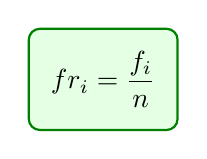
\begin{tikzpicture}
\node[rectangle, fill=green!10, rounded corners, inner sep=8pt, draw=green!50!black, thick] (box) {
$\displaystyle fr_i = \frac{f_i}{n}$
};
\end{tikzpicture}

\vspace{0.3cm}

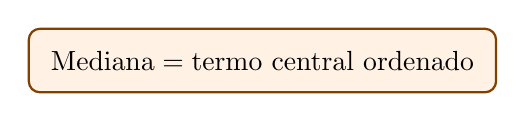
\begin{tikzpicture}
\node[rectangle, fill=orange!10, rounded corners, inner sep=8pt, draw=orange!50!black, thick] (box) {
$\displaystyle \text{Mediana} = \text{termo central ordenado}$
};
\end{tikzpicture}
\end{center}

\vspace{0.5cm}
\textcolor{blue}{\textbf{Legenda:}} 
\begin{itemize}
\item \textcolor{blue}{Respostas numéricas:} \respostaNum{exemplo}
\item \textcolor{blue}{Respostas textuais:} \textcolor{blue}{exemplo}
\end{itemize}

\atencao \textcolor{red}{Sempre verifique se a amostra é representativa antes de generalizar conclusões!}

\end{multicols}

\end{document}
